\section{Representación de los datos }
\label{sec:cap2-tecnicas-graficas-representacion}

Los objetos del mundo real se pueden describir mediante los fenómenos discretos y continuos. Las variables y
objetos se muestrean y organizan para lograr una representación adecuada. En un SIG existen básicamente dos
modelos lógicos que se conocen como formato raster y formato vectorial y que dan lugar a los dos grandes tipos
de capas de información espacial.

\subsection{Formato raster}
El formato raster o de retícula se centra en las propiedades del espacio más que en la precisión de la localización. Divide
el espacio en un conjunto regular de celdillas, cada una de estas celdillas contiene un número que puede ser el identificador
de un objeto o del valor de una variable.Se trata de un modelo de datos muy adecuado para la representación de variables
continuas en el espacio.

Los datos raster se compone de filas y columnas de celdas, cada celda almacena un valor único. Los datos raster pueden ser imágenes
con un valor de color en cada celda (o píxel de la imagen). Otros valores registrados para cada celda puede ser un valor discreto o
un valor nulo si no se dispone de datos. Si bien una trama de celdas almacena un valor único, estas pueden ampliarse mediante el
uso de las bandas del raster para representar los colores RGB (rojo, verde, azul), o una tabla extendida de atributos con una
fila para cada valor único de celdas. La resolución del conjunto de datos raster es el ancho de la celda en unidades sobre el
terreno.

\subsection{Formato vectorial}
Los datos vectoriales, se caracterizan por la precisión de localización de los elementos geográficos en el espacio, donde
los fenómenos a representar son discretos, con límites bien definidos. Generalmente se considera que el formato vectorial
es más adecuado para la representación de entidades o variables cualitativas y el formato raster para representar superficies.



\begin{figure}
\centering
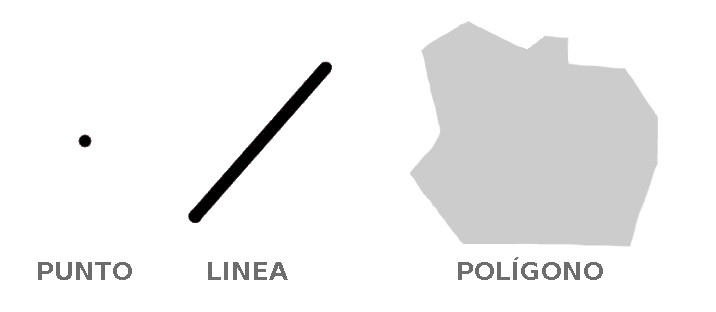
\includegraphics[width=0.6\textwidth]{capitulo-2/graphics/dimensiones-datos.jpg}
\caption{\label{fig:sig-xyz} Elementos geométricos utilizados para modelar digitalmente las entidades en un SIG.}
\end{figure}

Los diferentes objetos se encuentran representados como puntos, lineas o polígonos, donde cada una de estos elementos
geométricos se encuentra vinculado a una fila en una base de datos que describe sus atributos. De tal forma que para modelar
digitalmente las entidades del mundo real se utilizan estos tres elementos geométricos.
\begin{itemize}
    \item Puntos : se utilizan para las entidades geográficas que pueden ser descriptas por un único punto de referencia. Los
    puntos transmiten la menor cantidad de información, en los elementos puntuales no puede medirse la distancia. También
    se pueden utilizar para representar zonas a una escala pequeña.

    \item Líneas o polilíneas : las líneas unidimensionales o polilíneas son usadas para rasgos lineales como ríos,
    caminos, ferrocarriles, rastros, líneas topográficas o curvas de nivel. De igual forma que en las entidades
    puntuales, en pequeñas escalas pueden ser utilizados para representar polígonos. En los elementos lineales puede
    medirse la distancia.

    \item Polígonos : se utilizan para representar elementos geográficos que cubren un área particular de la superficie de la tierra.
    Los polígonos transmiten la mayor cantidad de información en archivos con datos vectoriales y en ellos se pueden medir el
    perímetro y el área.

\end{itemize}

\subsection{Ventajas y desventajas de los formatos raster y vectorial}
El debate acerca de la conveniencia de uno u otro modelo debe basarse en el tipo de estudio o enfoque que se quiera
hacer, pero también del software y fuentes de datos disponibles.

Está claro que las superficies se representan más eficientemente en formato raster y sólo pueden representarse
en formato vectorial mediante los modelos híbridos que no resultan adecuados para la realización de posteriores
análisis ya que todas las operaciones que permite el modelo ráster resultaran mucho más lentas con el modelo
vectorial.

Tradicionalmente se ha considerado que para la representación de los objetos resulta más eficiente la utilización
de un formato vectorial ya que La estructura de los datos es compacta y almacena los datos sólo de los elementos
digitalizados por lo que requiere menos memoria para su almacenamiento y tratamiento. Los elementos son representados
como gráficos vectoriales que no pierden definición si se amplía la escala de visualización. Sin emabargo el formato
vectorial es más lento, debido a su compleja estructura, que el raster para la utilización de herramientas de análisis
espacial y consultas acerca de posiciones geográficas concretas.

En el caso de las variables cualitativas estaríamos en un caso intermedio entre los dos anteriores.
Las ventajas del modelo ráster incluyen la simplicidad, la velocidad en la ejecución de los operadores y que es
el modelo de datos que utilizan las imágenes de satélite o los modelos digitales de terreno. Entre las desventajas
del modelo ráster destaca su inexactitud que depende de la resolución de los datos y la gran cantidad de espacio
que requiere para el almacenamiento de los datos. Este último problema puede compensarse mediante diversos
sistemas de compresión. Además en muchos casos se confunde precisión y exactitud cuando se trabaja con
datos vectoriales de modo que la exactitud en las coordenadas del modelo vectorial es más teórica que real.

Hoy en día se pueden codificar las formas en un modelo vectorial y los procesos con un modelo ráster,
para ello se requieren herramientas eficaces de paso de un formato al otro. Resulta sencillo, finalmente, la
visualización simultánea de datos en los dos formatos gracias a la capacidad gráfica actual.
